\section{Force of Infection}\label{sr.foi}
This section presents supplementary results and commentary regarding
force of infection equations and assumptions.
%===================================================================================================
\subsection{Inert Sex Act Proportion}\label{sr.foi.inert}
Figure~\ref{fig:binom.inert} illustrates
the proportion of sex acts which are modelled as inert per \eqref{eq:inert}, which increases with
the total number of sex acts $A$ and
the probability of transmission per act $\beta$.
\begin{figure}[h]
  \centering\includegraphics[scale=1]{binom.inert}
  \caption{Proportion of sex acts which are modelled as inert}
    \label{fig:binom.inert}
  \floatfoot{
    $B$: probability of transmission per partnership;
    $\beta$: probability of transmission per act;
    $A$: total acts per partnership.}
\end{figure}
%===================================================================================================
\subsection{Proof that $B_{\wph} \ge B_{\bph}$}\label{sr.foi.proof}
In \sref{foi.prior.bhom}, we claimed that
the per-partnership probability of transmission $B$ is larger for
within- \vs between-partnership heterogeneity
--- $B_{\wph} \ge B_{\bph}$, from \eqrefs{eq:B.wph}{eq:B.bph}, respectively ---
given the same set of transmission modifiers $R_f, \alpha_f$.
Here is a proof of that claim:
\begin{equation}
  \begin{aligned}
    B_{\wph} &\ge B_{\bph} \\
    1 - \prod_f {(1 - \beta_f)}^{A\alpha_f} &\ge 1 - \sum_f \alpha_f {(1 - \beta_f)}^{A}
  \end{aligned}
\end{equation}
Let $x_f = {(1 - \beta_f)}^A$; then
\begin{equation}\label{eq:AM-GM}
  \prod_f {x_f}^{\alpha_f} \le \sum_f \alpha_f x_f
\end{equation}
Since $\sum_f \alpha_f = 1$ and $\alpha_f \in [0,1]$ are effectively weights,
\eqref{eq:AM-GM} is the weighted arithmetic mean--geometric mean (AM-GM) inequality \cite{Aldaz2009}.
\citet{Aldaz2009} further shows that the gap between $B_{\wph}$ and $B_{\bph}$
increases with the $\alpha_f$-weighted variance in ${\beta_f}^{\frac12}$
(though the proportionality is not exactly linear),
which supports the results of \sref{foi.exp.xph} mathematically.
\par
Using Jensen's inequality \cite{Jensen1906} we can also show that
the approach in \cite{Kerr2015} (and others)
to aggregate heterogeneity by HIV infection stage first
produces an intermediate per-partnership probability $B_{\xph}$:%
\footnote{\hreftt{math.stackexchange.com/q/4660409}}
\begin{equation}
  B_{\wph} \ge B_{\xph} \ge B_{\bph},
  \qquad B_{\xph} = 1 - {(1 - \sum_f \alpha_f \beta_f)}^{A}
\end{equation}
%===================================================================================================
\subsection{Alternate Modelling Frameworks}\label{sr.foi.alt}
Recognizing the limitations of compartmental models in simulating
infectious disease transmission via sexual partnerships,
two main alternate modelling frameworks have been developed \cite{Rao2021}.
These frameworks are illustrated in Figure~\ref{fig:fw}.
Modelling frameworks are further classified Appendix~1 of \cite{Johnson2016mf}.
\begin{figure}[b]
  \centering\foreach \var/\cap in
  {comp/Classic compartmental,pair/Pair-based,ibm/Individual-based}{%
  \begin{subfigure}[b]{.33\linewidth}
    \centering
    \includegraphics[width=.9\linewidth]{mf.\var}
    \caption{\cap}
    \label{fig:mf.\var}
  \end{subfigure}}
  \caption{Representations of health states and sexual partnerships
    under 3 different STI modelling frameworks}
  \label{fig:fw}
  \floatfoot{
    $S$: susceptible; $I$: infectious;
    solid arrows: partnerships; dashed arrows: state transitions.}
\end{figure}
%---------------------------------------------------------------------------------------------------
\paragraph{Pair-Based Models}
Pair-based models, also known as pair-formation models, were developed as early as 1988,
with the explicit motivation to overcome limitations of
classic compartmental models of STI transmission \cite{Dietz1988sti}.
In pair-based models, the fundamental population stratification
reflects different partnership configurations and health states \cite{Kretzschmar2017}, such as:
susceptible and single, a susceptible/infected pair in a long-term partnership, etc.
(Figure~\ref{fig:mf.pair}).
Such models can therefore track the numbers of partnerships
where transmission is \vs is not possible,
thereby avoiding the instantaneous partnership assumption.
Pair-based models have been applied to a variety of STIs \cite{Kretzschmar2017}.
However, the numbers of compartments required to reflect all possible partnership configurations
\emph{and} all possible health states among connected partners
quickly become impractical \cite{Kretzschmar2017,Rao2021}.
For example, a classic compartmental model with 2 risk groups and 2 health states
would require $2\times2=4$ compartments;
whereas even a first-order pair-based model (\ie without ``triples'')
would require $2\times2$ (singles) + ${(2\times2)}^2$ (pairs) ${} = 20$ compartments;
a second-order pair-based model (\ie with ``tripples'')
would require $4 + 4^2 + 4^3 = 84$ compartments.
Thus, pair-based models are especially limited in their ability to model partnership concurrency
--- the role of which in HIV epidemiology remains controversial \cite{Sawers2013}.
As such, pair-based models have seen little widespread adoption
for HIV transmission modelling~\cite{Rao2021}.
If long-term concurrency is rare, a hybrid approach is possible,
wherein long-term pairs are explicitly modelled,
but additional ``one-off'' partnerships are modelled as instantaneous~\cite{Xiridou2003,Powers2011ahi}.
%---------------------------------------------------------------------------------------------------
\paragraph{Individual-Based Models}
Individual-based models, also knowns as agent-based, network-based, or microsimulation models,
explicitly simulate unique individuals (Figure~\ref{fig:mf.ibm}).
They represent a fundamental change in the model unit from groups of individuals
--- \ie the ``compartments'' of compartmental models \cite{Rao2021}.
Individual-based models can therefore model unique partnerships, and track them over time.
Such individuals and partnerships can then be
parameterized in fundamentally different ways \vs compartmental models,
including with continuous valued features like infection age and sex frequency,
\vs predetermined categories like infection stages and partnership types \cite{Pellis2015,Rao2021}.
Parameters for each individual and partnership are thus sampled randomly and/or dynamically,
allowing more complete and nuanced representations of risk heterogeneity and partnership dynamics.
Such nuances can in fact be key determinants of epidemic dynamics and intervention impact
\cite{Hontelez2013,Johnson2016mf}.
Evidently, many of the limitations of compartmental and pair-based models
do not apply to individual-based models \cite{Rao2021}.
Yet these limitations are replaced with new challenges,
especially related to implementing, parameterizing, and calibrating these powerful models
\cite{Rao2021,Pellis2015,Hazelbag2020}.
For example, much effort has been dedicated to
formalizing the statistical properties of dynamic networks
via temporal exponential family random graph models (tERGM) \cite{Jenness2018}
or latent order logistic models (LOLOG) \cite{Clark2022},
so that dynamic networks can be generated which are consistent with observed data.
Although individual-based models have seen greater use than pair-based models,
these challenges still prevent universal adoption over classic compartmental models \cite{Rao2021}.
It's worth noting that not all individual-based models are transmission models,
as individual-based models can also be used for
simulation and inference for non-infectious diseases~\cite{Silverman2021}.
%===================================================================================================
\subsection{Illustrative Scenario Motivating the Proposed Approach}\label{sr.foi.toy}
Consider the moment of one transmission event
in a population of 16 monogamous partnerships, with 25\% infection prevalence
and random mixing by infection status (Figure~\ref{fig:foi.toy.pair}).
Initially, infection prevalence is equal among partners of
susceptible $S$ and infectious $I$ individuals: 6/24 and 2/8, respectively.
Immediately after transmission,
prevalence decreases to 5/23 among partners of $S$ but increases to 4/9 among partners of $I$,
decreasing the population-level transmission risk.
Next, three events are possible:
\begin{enumerate}
  \item[(a)] \label{toy.e.t}
  another transmission occurs among the remaining $S$-$I$ partnerships,
  yielding 4/22 prevalence among partners of $S$, and 6/10 among partners of $I$;
  population-level transmission risk decreases further
  \item[(b)] \label{toy.e.p}
  the partnership from the original transmission ends,
  and both individuals form new partnerships (assumed at random),
  yielding, on average, 9/32 prevalence among partners of both $S$ and $I$;
  population-level transmission risk increases \emph{above} the initial level ($9/32 > 6/24$)
  \item[(c)] \label{toy.e.q}
  any other partnership ends,
  and both individuals form new partnerships (assumed at random);
  infection prevalence among $S$ and $I$, and population-level transmission risk
  all remain unchanged, on average
\end{enumerate}
Prior compartmental models have effectively assumed that
event (b) always occurs before (a)
--- \ie the ``instantaneous partnership assumption''.
This assumption is reflected in Figure~\ref{fig:foi.toy.freq},
where the frequentist approximation does not explicitly model any individual partnerships.
This assumption is evidently worse for longer partnerships.
\begin{figure}
  \begin{subfigure}{.5\linewidth}
    \centering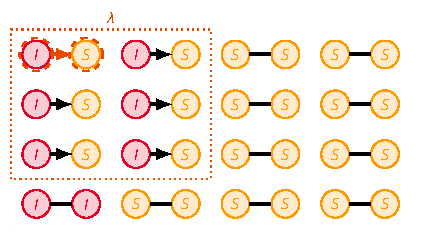
\includegraphics[scale=1]{foi.toy.pair}
    \caption{Pair-wise reality}
    \label{fig:foi.toy.pair}
  \end{subfigure}%
  \begin{subfigure}{.5\linewidth}
    \centering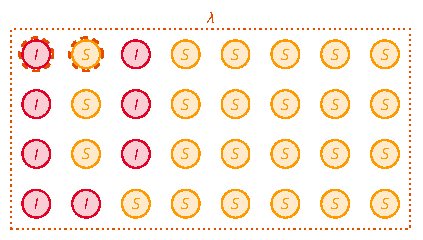
\includegraphics[scale=1]{foi.toy.freq}
    \caption{Frequentist approximation}
    \label{fig:foi.toy.freq}
  \end{subfigure}
  \caption{Comparison of pair-based reality and frequentist approximation
    for a population of 16 pairs with 25\% infection prevalence,
    at the moment of one transmission event}
  \label{fig:foi.toy}
  \floatfoot{
    $S$: susceptible; $I$: infectious; $\lambda$: force of infection;
    dashed circles: individuals involved in transmission event.}
\end{figure}
%===================================================================================================
\subsection{Calibration under Different Force of Infection Approaches}\label{sr.foi.cal}
This section presents supplementary results of Eswatini model calibration
under the 4 force of infection approaches explored in \sref{foi.exp.model}:
Effective Partnerships Reduction (\epa),
Instantaneous Rate-Duration (\ird),
Instantaneous Rate-1-Year (\iry), and
Instantaneous Proportion-1-Year (\ipy).
\par
Figure~\ref{fig:ll.hist.foi} illustrates
the distributions of log likelihoods for 1000 model fits under each approach, while
Figure~\ref{fig:post.distr.foi} illustrates
the corresponding distributions of calibrated model parameters.
\begin{figure}
  \centering\includegraphics[scale=1]{ll.hist.foi}
  \caption{Distribution of log likelihoods across force of infection approaches}
  \label{fig:ll.hist.foi}
  \floatfoot{\fffoi.}
\end{figure}
\begin{figure}
  \centering\includegraphics[width=\linewidth]{post.distr.foi}
  \caption{Posterior distributions of calibrated model parameters,
    under different force of infection approaches (colours)}
  \label{fig:post.distr.foi}
  \floatfoot{\ffpar; \fffoi; \ffpost;
    \ffast{QN rank score test \cite{Kruskal1952} for comparing distributions}}
\end{figure}
\par
Figures~\ref{fig:fit.prev.foi}--\ref{fig:fit.inc1v2.foi} illustrate the modelled HIV
prevalence, prevalence ratios, incidence, and incidence ratios,
plus associated calibration targets, for each approach.
Qualitative differences between approaches appear to be minimal,
except for lower incidence among FSW in Figure~\ref{fig:fit.inc.foi-py},
as expected (see \sref{foi.exp.mod.dyn}).
\par
\foreach \vf/\var/\vlab in {%
  1/prev/prevalence,%
  1/prev1v2/prevalence ratios between selected risk groups,%
  1/inc/incidence,%
  .6/inc1v2/incidence ratios between selected risk groups}{
  \begin{figure}[h]
    \subcapoverlap\centering
    \foreach \foi in {base,foi-rd,foi-ry,foi-py}{
      \begin{subfigure}{\vf\linewidth}
        \centerline{\includegraphics[scale=\fitscale]{fit.\var.\foi.all}}
        \caption{\raggedright}
        \label{fig:fit.\var.\foi}
      \end{subfigure}\\}
    \caption{Modelled HIV \vlab and associated calibration targets
      under different force of infection approaches}
    \label{fig:fit.\var.foi}
    \floatfoot{Approaches:
      \foreach \foi/\flab in {base/\epa,foi-rd/\ird,foi-ry/\iry,foi-py/\ipy}{
        \sfref{fig:fit.\var.\foi}: \flab;}
      \fffoi; \fffit; \ffribbon; \ffpbar.}
  \end{figure}}
\par
Finally, Figure~\ref{fig:foi.wiw.ptr} illustrates
the proportions of modelled yearly HIV infections
transmitted via different partnership types under each approach, with
equal parameters (calibrated under \epa, top row) and
approach-specific parameters (recalibrated, bottom row).
\begin{figure}[h]
  \includegraphics[width=\linewidth]{foi.wiw.ptr}
  \caption{Proportions of modelled yearly HIV infections
    transmitted via different partnership types in Eswatini
    estimated under different force of infection approaches (horizontal facets)
    with equal \vs approach-specific parameters (vertical facets)}
  \label{fig:foi.wiw.ptr}
  \floatfoot{\fffoi; \ffwiw.}
\end{figure}
